%!TEX root = ../bare_jrnl.tex

\section{Evaluation on Aggregate Human Occupancy Behaviour Dataset}
\label{sec:evareal}

We now investigate the performance of the POPP model and its extensions on a real world dataset\footnote{The dataset can be downloaded from \url{https://github.com/ferdianjovan/spectral_popp}}.
% 
The dataset was gathered from an office building in which a mobile robot~\cite{hawes2016strands} counted the number of people in different regions whilst patrolling (see Figure~\ref{fig:map_popp_independent_test} for the map of the building). The dataset contains time series  counts from three different automated person detectors~\cite{dondrup2015real}. These use laser, depth camera and RGB information. We refer to these detectors respectively as the leg detector (LD), upper body detector (UBD), and change detector (CD). Each of these detectors acts as one sensor. Each returns a sensed count of the number of people it detected in each 10 minute interval during the day. These detectors are unreliable, as can be seen from Figure~\ref{fig:single_sensor_rate_transformation}, which shows examples of correct and incorrect detections.

\begin{figure}[t]
	\centering
	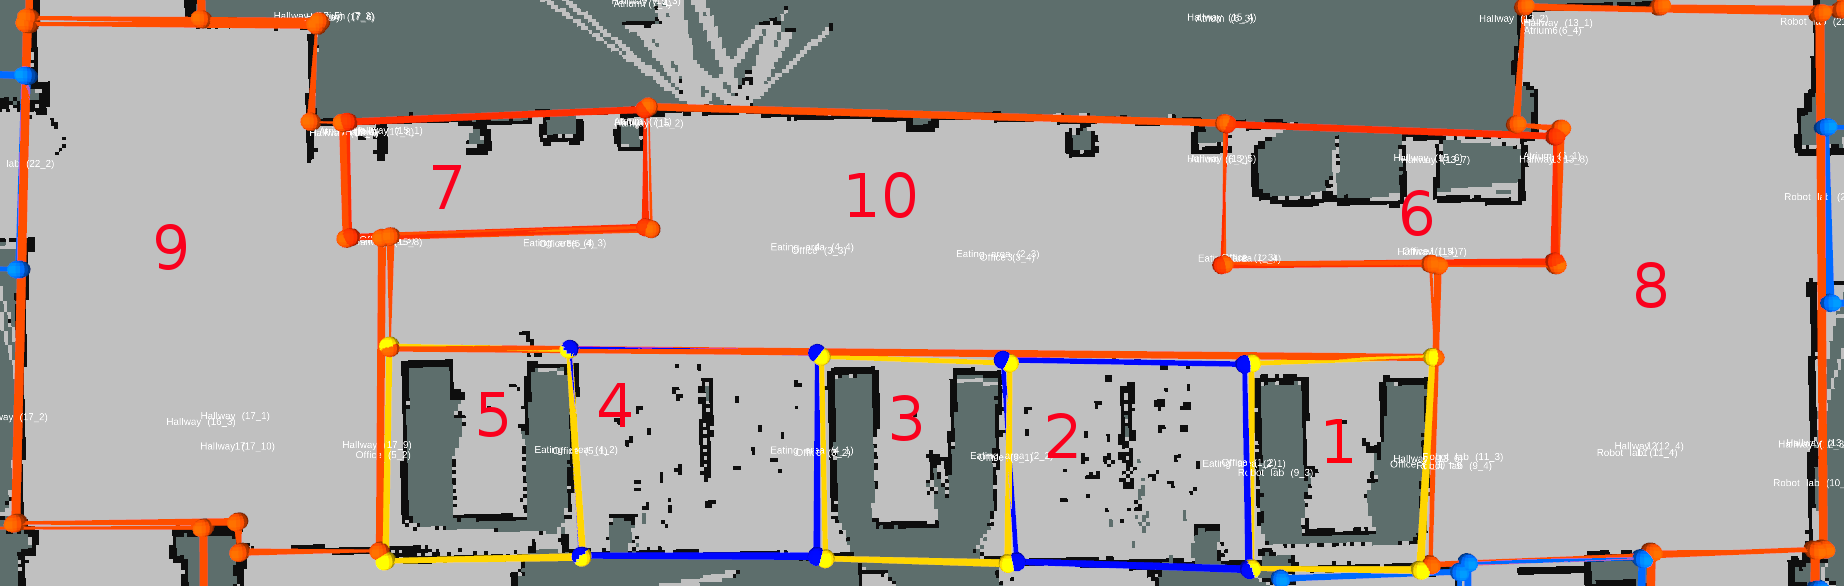
\includegraphics[width=0.95\columnwidth]{./figures/map_popp.png}
	\caption{The office building in which the robot gathered data. Areas are bounded by imaginary lines.}
	\label{fig:map_popp_independent_test}
\end{figure}

\begin{figure}[t]
	\centering
	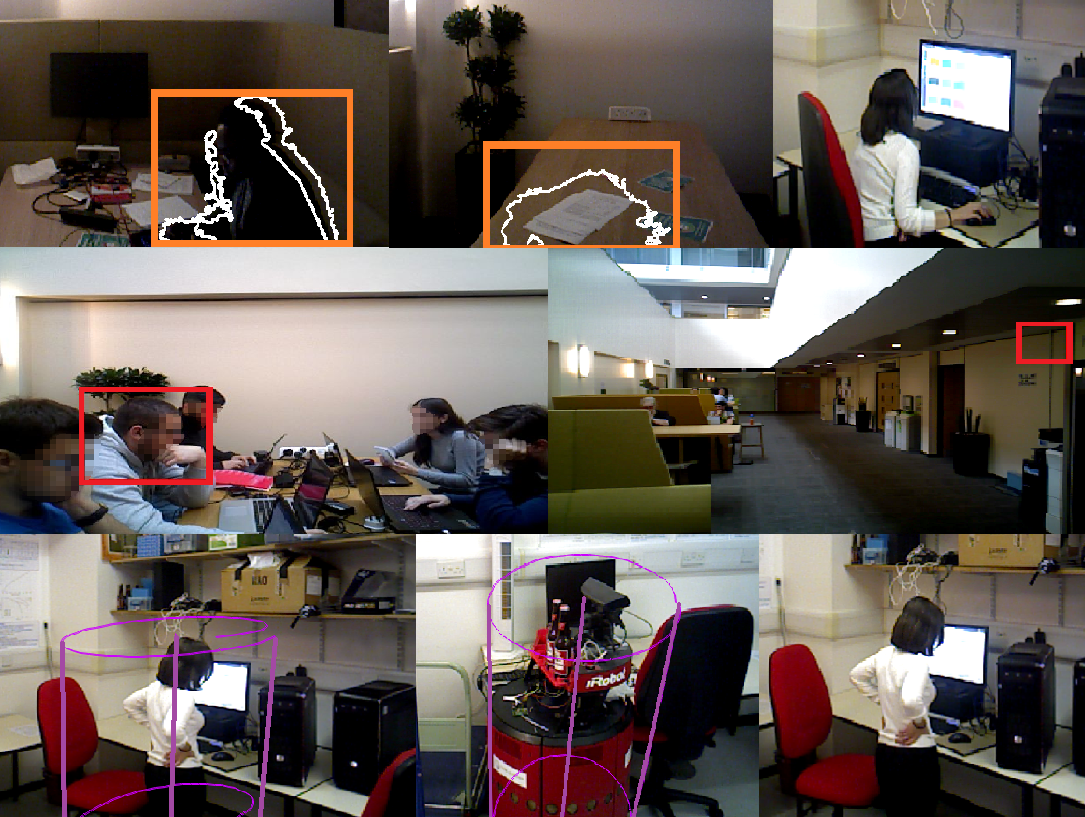
\includegraphics[width=0.95\columnwidth]{./figures/sensor_images.png}
	\caption{Correct and incorrect detections, and non-detections, from different regions in the environment for each sensor. Top row: change detector. Middle row: upper body detector. Bottom row: leg detector. Detections are marked with 2D or 3D bounding boxes. A bounding box containing a person is a correct detection (true positive). One without a person is an incorrect detection (false positive). A person without a bounding box is a missed detection (false negative).}
	\label{fig:single_sensor_rate_transformation}
\end{figure}

By comparing the ground truth with the detections made by sensors, we compute a sensor model for each region. An average of the sensor models across all regions can be seen in Table \ref{table:sensor_model_popp_beta}. Although the robot operated for 24 hours day, the sensor models were built using only the data collected from 10am to 8pm, since there were few detections outside these times. From a 69 day trial of the mobile robot, we obtained 48 days of usable observations. We specified a time interval for each Poisson distribution of 10 minutes, and recorded both the true counts and the detections made by each sensor in each interval. We assumed the underlying process in each region to be a periodic Poisson process in which there is a one-day periodicity, i.e. $\lambda(t) = \lambda(t + \Delta)$ with $\Delta = 24 * 60$ (minutes). This means that the expected number of people each day at a particular time is expected to be the same across the 48 days of observations. We estimated the true parameter $\lambda'(t)$ of the Poisson distribution at $t$ by running a FOPP model on the true counts within each interval. We use this estimate of $\lambda'(t)$ from the true counts as the target which the POPP models must estimate from the sensed counts.

The different POPP approaches rely on sensor models that must be calculated from a confusion matrix relating true counts to the sensed counts from the different sensors. To separate the training and testing data we performed four fold cross-validation with data splits being on whole days, i.e., we used 12 days of data as a training set for a sensor model and then used the remaining 36 days of data as a test set on which to test the inferences made by each model from the sensor counts.

\begin{table}[t]
	\centering
	\caption{Averaged sensor models across all areas trained from 48 days of data.}
	\label{table:sensor_model_popp_beta}
	\begin{tabular}{lccc}
		\noalign{\hrule height 1.1pt}\noalign{\smallskip}
		Sensor & True Positive & True Negative \\
		\noalign{\smallskip}\hline\noalign{\smallskip}
		Leg Detector & 0.387 & 0.951 \\
		Upper Body Detector & 0.356 & 0.882 \\
		Change Detector & 0.731 & 0.900 \\ 
		\noalign{\hrule height 1.1pt}\noalign{\smallskip}
	\end{tabular}
\end{table}

For the 36 days of test data, the different models each made predictions of the $\lambda(t)$ parameter of the Poisson. Given this, we recorded (1) the RMSE between the MAP hypothesis of each model posterior distribution over $\lambda(t)$ and the true $\lambda'(t)$ and (2) the Jensen-Shannon distance between the posterior distribution $P(\lambda(t) \mid \mathbf{s_i})$ and the distribution of the true $\lambda'(t)$. Using these metrics, we compared the performance of all POPP models (estimated using the switching filter described in~\ref{sec:estimators}) to the Bayes' filter arising from the FOPP model. The FOPP model is a single sensor model and was estimated from the change detector counts since this was the most reliable detector among the three available (as shown in Table~\ref{table:sensor_model_popp_beta}). 

Figures \ref{fig:fopp_popp_popb_npop_popd_rmse_evo} and \ref{fig:fopp_popp_popb_npop_popd_kl_evo} show the accuracy comparison between all POPP models and the standard FOPP model over time. It can be seen that all models become more accurate as the days pass. All POPP models show more accuracy over the standard FOPP model. The $\lambda(t)$ estimate produced by the POPP-Dirichlet model is more accurate than the ones produced by the standard POPP model and the POPP-Beta model. However, the POPP-Dirichlet estimate is not always more accurate than the one produced by the C-POPP model. 

As the POPP-Dirichlet model is more conservative in estimating the parameter $\lambda(t)$ than the C-POPP model, the estimate moves more slowly towards the true $\lambda'(t)$. This is seen in Figure~\ref{fig:fopp_popp_popb_npop_popd_kl_evo}.
By the third day, the POPP-Dirichlet model outperformed the POPP, POPP-Beta, and C-POPP models in terms of accuracy. However, the accuracy gap between the C-POPP model and the POPP-Dirichlet model becomes smaller over time. By the 36th day the C-POPP model outperforms the POPP-Dirichlet by a small margin. It should be noted that Figures \ref{fig:fopp_popp_popb_npop_popd_rmse_evo} and \ref{fig:fopp_popp_popb_npop_popd_kl_evo} are averaged RMSE and the Jensen-Shannon distance from 10 different regions over time. The more regions with high volume of data available, the more accurate the joint sensor model, especially for C-POPP, will be and, in turns, the more accurate the C-POPP filter becomes in estimating the parameter $\lambda(t)$.

\begin{figure}[t!]
	\centering
	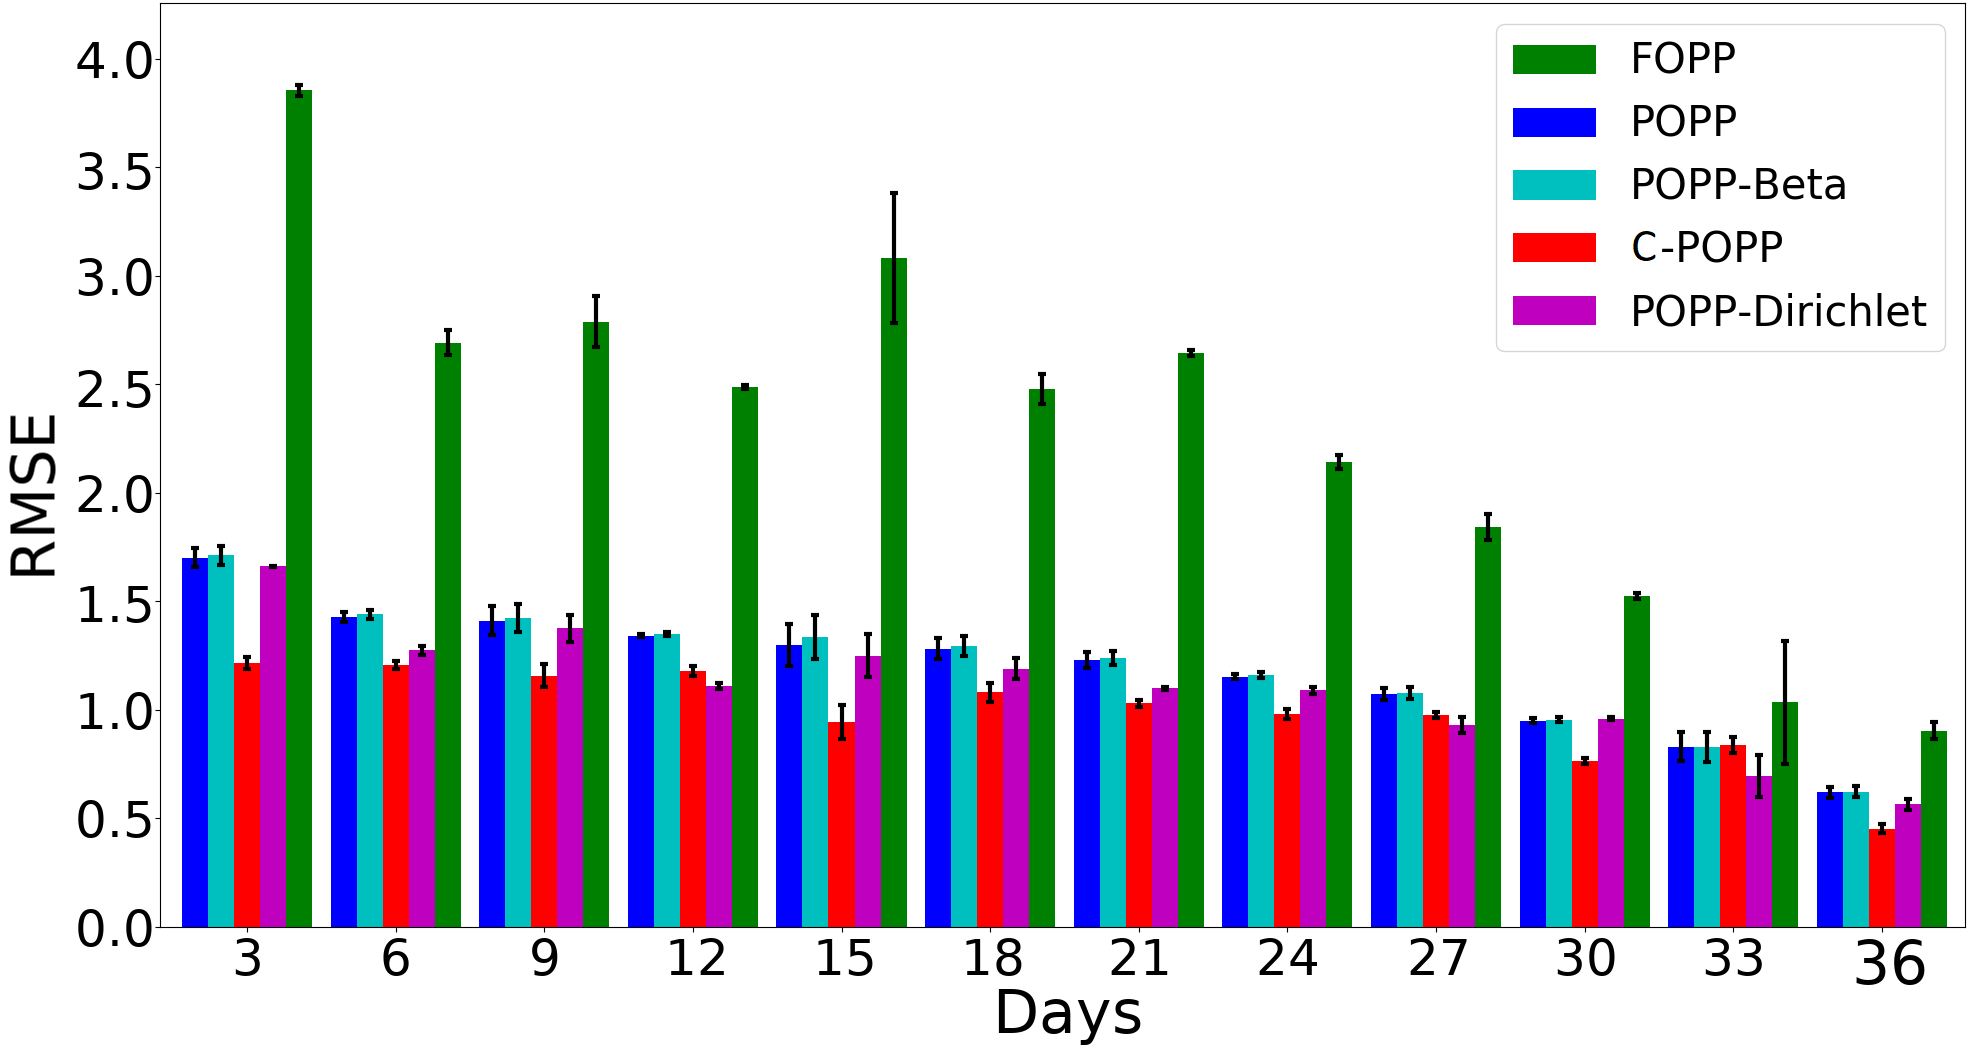
\includegraphics[width=0.95\columnwidth]{./figures/fopp_popp_popb_npop_popd_rmse_evo.png}
	\caption{The RMSE evolution of periodic Poisson processes with POPP, POPP-Beta, C-POPP, POPP-Dirichlet and FOPP filters from day 3 to day 36, averaged across all regions. Standard error is shown.}
	\label{fig:fopp_popp_popb_npop_popd_rmse_evo}
\end{figure}

\begin{figure}[t!]
	\centering
	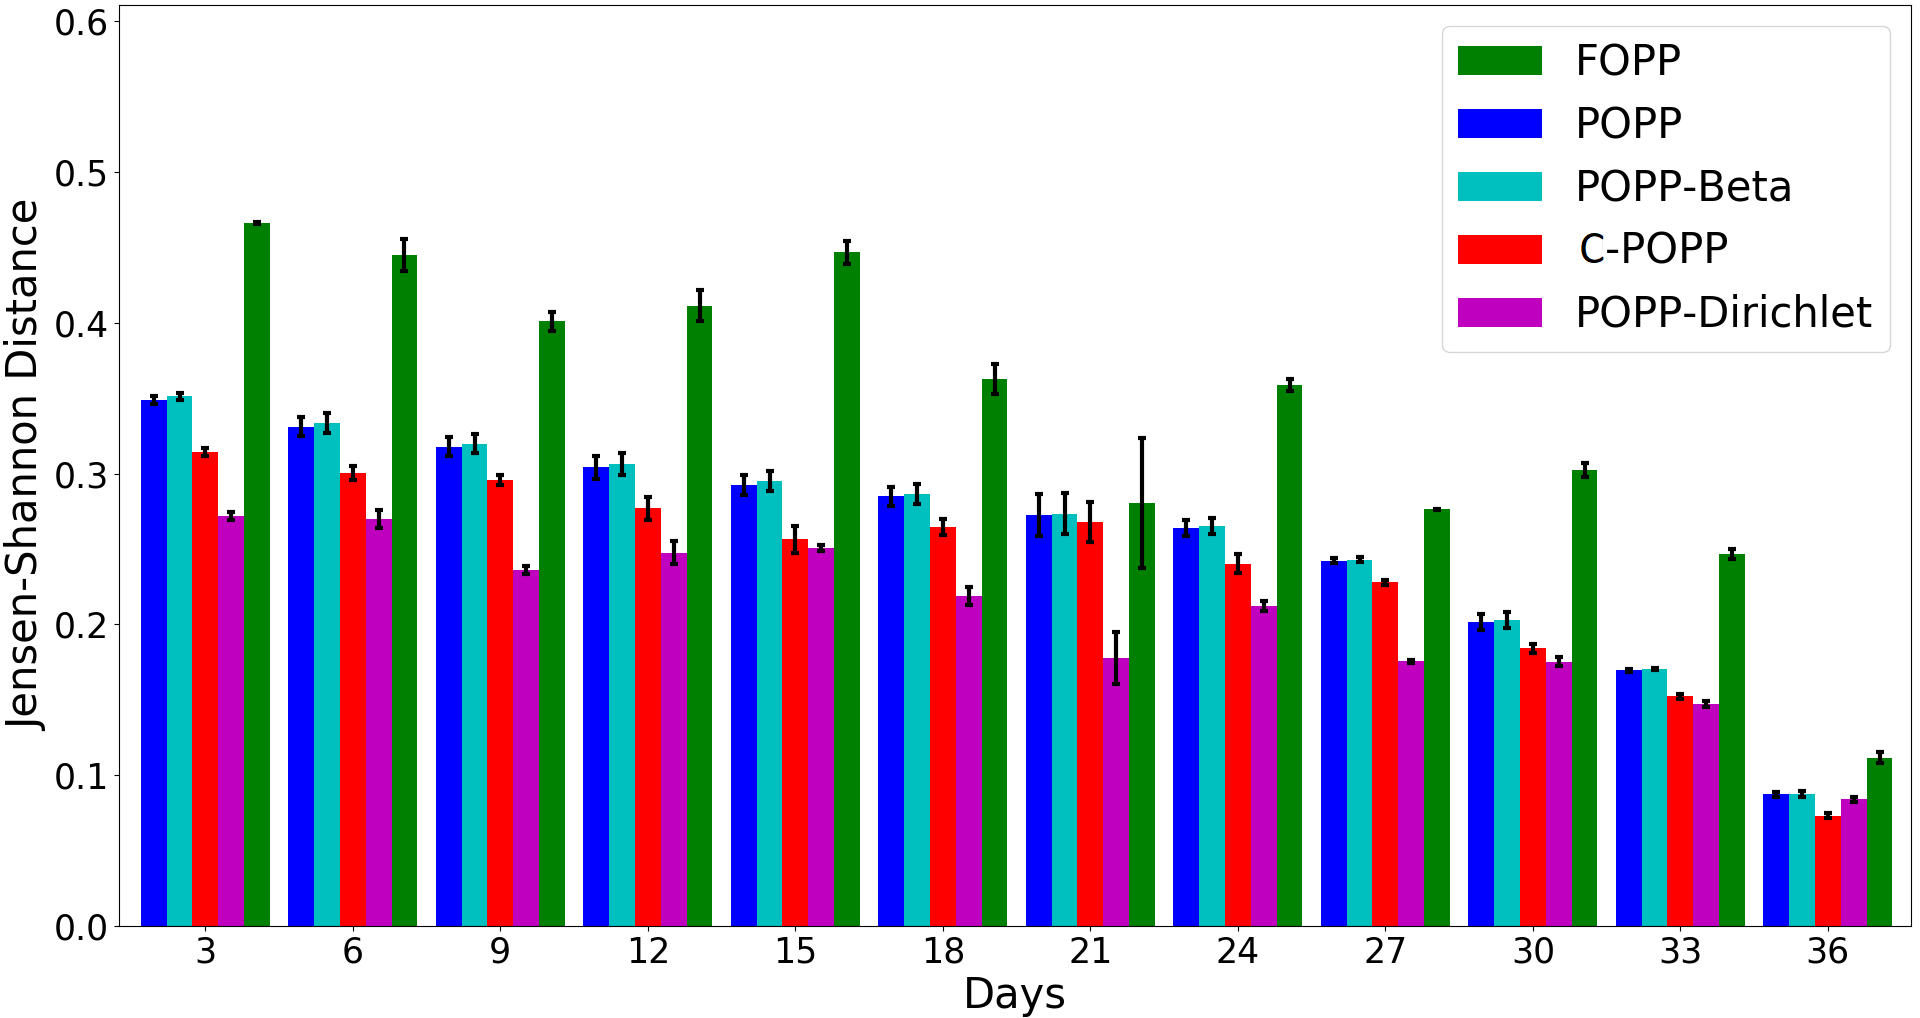
\includegraphics[width=0.95\columnwidth]{./figures/fopp_popp_popb_npop_popd_kl_evo.png}
	\caption{The Jensen-Shannon distance evolution of the FOPP, the POPP, the POPP-Beta, the C-POPP, and the POPP-Dirichlet filters in periodic Poisson processes from day 3 to day 36 in a 3-day interval, averaged across all regions. Standard error is shown.}
	\label{fig:fopp_popp_popb_npop_popd_kl_evo}
\end{figure}

\begin{figure}[t!]
	\centering
	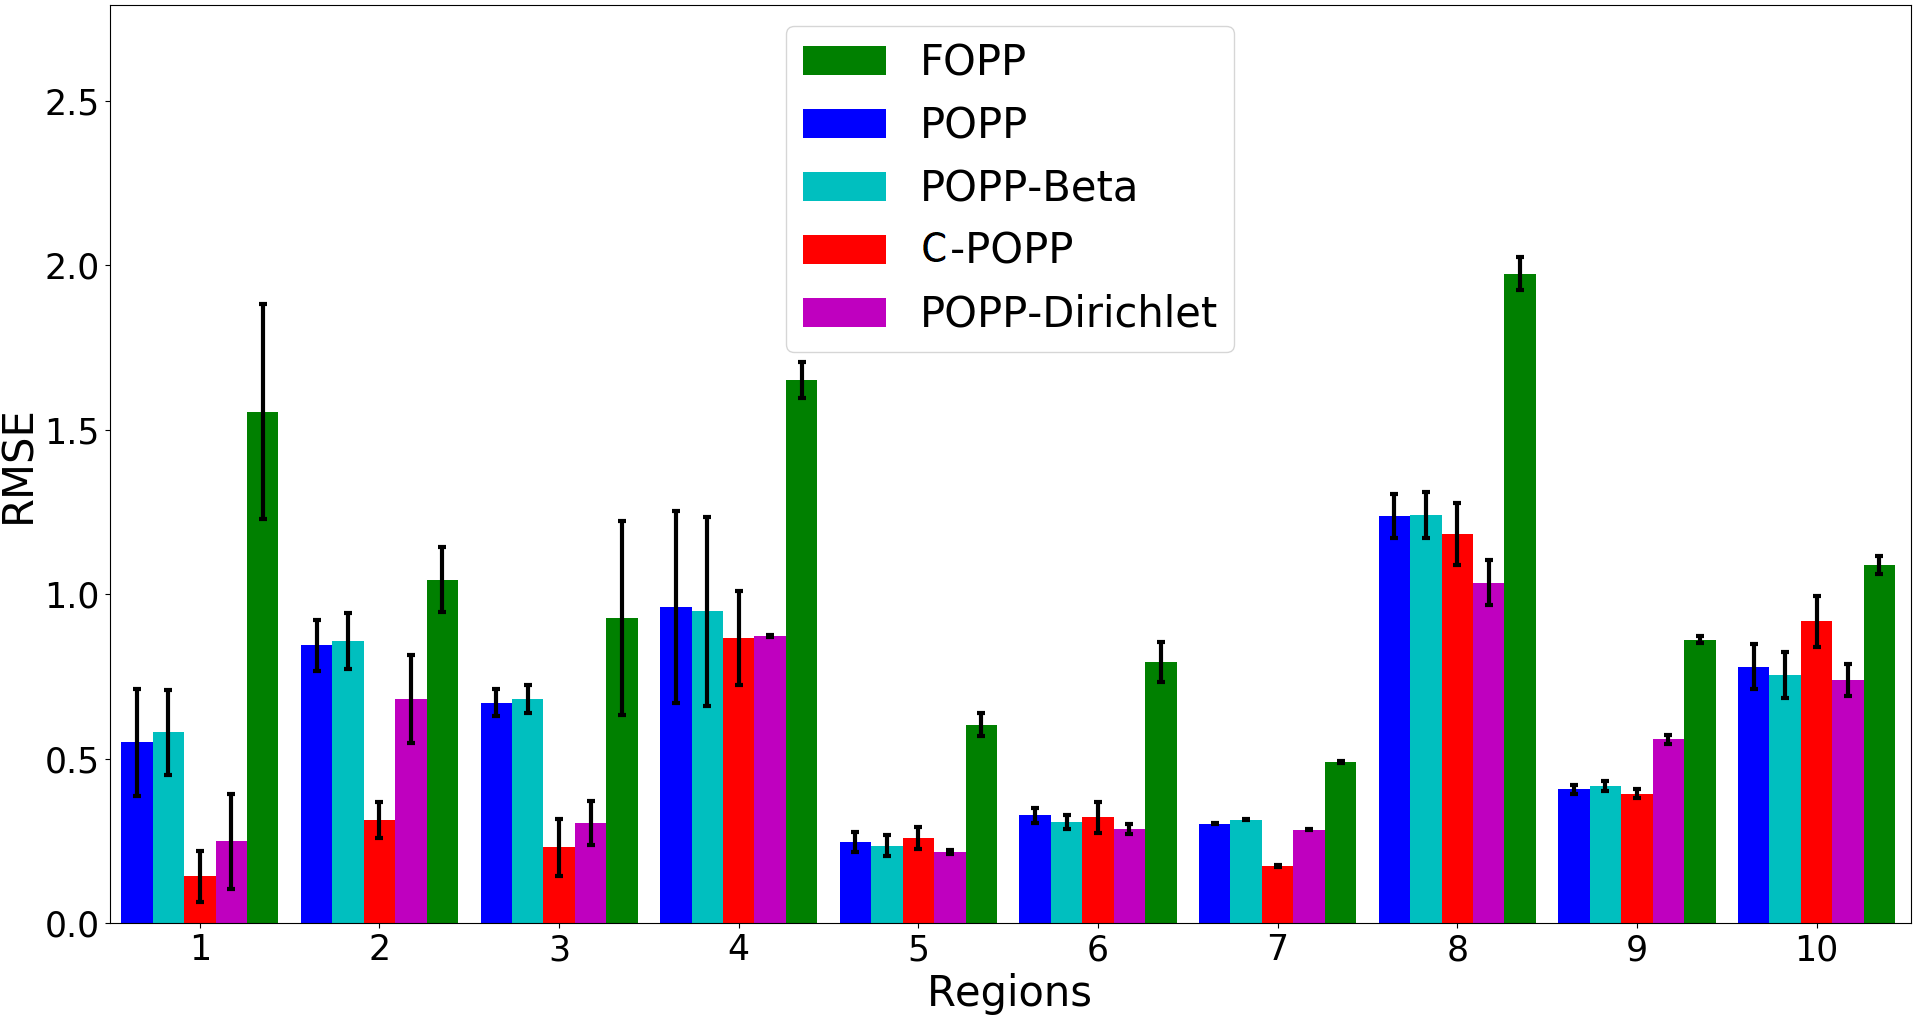
\includegraphics[width=0.95\columnwidth]{./figures/fopp_popp_popb_npop_popd_rmse.png}
	\caption{The RMSE of the FOPP, POPP, POPP-Beta, C-POPP, and POPP-Dirichlet filters across regions. The RMSE(s) are taken at the 36th day. Standard error is shown.}
	\label{fig:fopp_popp_popb_npop_popd_rmse}
\end{figure}

\begin{figure}[t!]
	\centering
	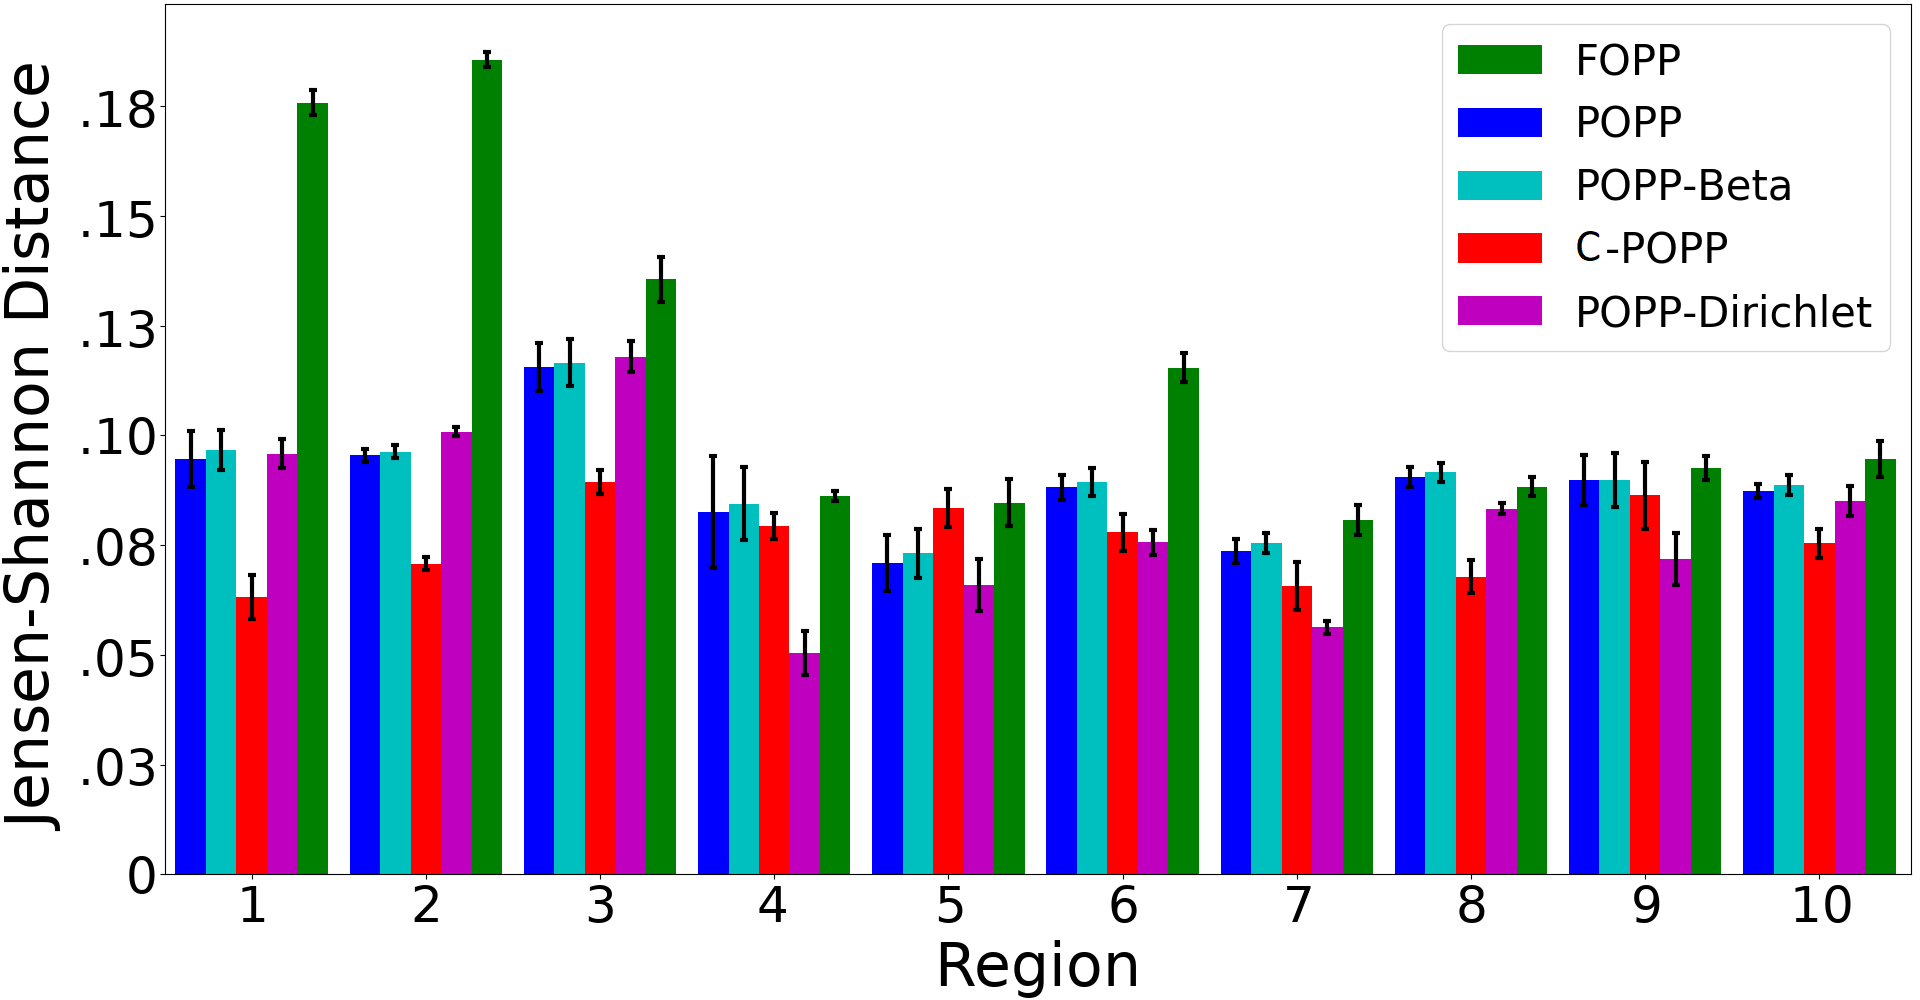
\includegraphics[width=0.95\columnwidth]{./figures/fopp_popp_popb_npop_popd_kl.png}
	\caption{The Jensen-Shannon of the FOPP, POPP, POPP-Beta, C-POPP, and POPP-Dirichlet filters across regions. The Jensen-Shannon value(s) are taken at the 36th day. Standard error is shown.}
	\label{fig:fopp_popp_popb_npop_popd_kl}
\end{figure}

Figure \ref{fig:fopp_popp_popb_npop_popd_rmse} and \ref{fig:fopp_popp_popb_npop_popd_kl} show the RMSE and Jensen-Shannon comparison between all POPP models and the FOPP across different regions by the end of the 36th day. It can be seen that the POPP-Dirichlet and the C-POPP once again outperformed the other models. Some regions such as 1, 2, and 3 have much more data than other regions. Since this  provides  more data to create the sensor models than other regions, the point-estimate joint sensor model for the C-POPP filter can be more accurately estimated for these regions. Unlike C-POPP filter, the POPP-Dirichlet estimates the joint sensor model as a distribution. This drives the POPP-Dirichlet slower and more conservative in estimating the parameter $\lambda(t)$ than the C-POPP model. Together with the choice of Dirichlet prior that follows uniform distribution, the POPP-Dirichlet requires more data to accurately estimate its joint sensor model.

The POPP-Dirichlet has an advantage on regions with low volume of data such as region 4, 5, 6 and 7. As some of these data were used to construct the joint sensor model for both C-POPP and the POPP-Dirichlet, a small amount of data creates an inaccurate point-estimate joint sensor model, which is used by the C-POPP filter. These problem is handled appropriately on the POPP-Dirichlet with its distribution joint sensor model with the help of Dirichlet prior as explained in Section \ref{subsec:popd}.

One interesting finding here is that there is small to no difference in performance between the POPP and the POPP-Beta filters on region 4, 5, 6, and 7. One would have thought that the performance of these two filters should follow the C-POPP and the POPP-Dirichlet filters. We argue that the volume of data used to create the sensor models for both POPP and the POPP-Beta were enough for an accurate estimate of point-estimate sensor model (POPP) and distribution sensor model (POPP-Beta). However, due to high correlations among sensors which were not captured by both the POPP and the POPP-Beta sensor models, the accuracy in estimating the parameter $\lambda(t)$ is worse than the C-POPP and the POPP-Dirichlet. For example, region 4 contains high tables and tall chairs where the leg detector tended to falsely detected them as a person. Unless an upper body detector detects a person, the leg detector detection may be ignored. On the other hand, region 7 is a hallway with a water dispenser around the corner. This water dispenser is often falsely detected as a person by the upper body detector and the leg detector detections helps in reducing this mistake.

% One should remember there are only six hyperparameters needed estimate for the sensor model in the POPP and the POPP-Beta compared to sixteen hyperparameters needed estimate for the joint sensor model in the C-POPP and the POPP-Dirichlet. 

%Similar to the C-POPP model, the POPP-Dirichlet model is able to cope and overcome the problems with limited sample data both for building the joint sensor model and estimating the $\lambda(t_i, t_j)$. In many regions, the POPP-Dirichlet managed to show better estimates as well as more similar distributions than the POPP, the POPP-Beta, and the FOPP models. However, the POPP-Dirichlet filter falls behind both in accuracy (RMSE) and distribution similarity compared to the C-POPP model. This is attributed to the POPP-Dirichlet conservative way in estimating the parameter $\lambda(t_i, t_j)$ compared to the C-POPP model.